\chapter{An introduction to RNA bioinformatics and pathogen genomics}
\label{chap:intro}
\section{Preface}
Bacteria are the most diverse and abundant type of organism on the planet \citep{Hug2016-nr}. Among the multitude of possible evolutionary niches, only a small subset of bacteria occupy pathogenic roles \citep{noauthor_2011-sb,Balloux2017}. Bacterial pathogens exhibit a remarkable range of adaptions to survive stresses encountered both in the environment and within the host. These include the acquisition of new genes \textit{via} horizontal transfer \citep{Kado2009-eh,Groisman1996-fv}, as well as changes in both gene function \citep{Moxon1994-oe} and gene expression \citep{Thomas2014-ln}.
Despite having far fewer genes than eukaryotes, sophisticated regulatory networks allow bacteria to sense and respond to their environment \citep{Dorman2018-dv}. The regulatory function and evolution of many non-coding RNAs (ncRNAs) have been identified as major contributors to the virulence and survival of many bacterial pathogens \citep{Gottesman2005-cp,Gripenland2010-rm}. Of particular interest are the small non-coding RNAs (sRNAs) that participate in regulatory networks \textit{via} interactions with mRNA and proteins \citep{Gottesman2011-vx}.\par

This thesis will primarily focus on the technicalities of identifying and studying non-coding RNA sequences in bacterial pathogens. Specifically, within the genus \textit{Salmonella} and other pathogens of the Enterobacteriaceae that infect animals and plants, and the kiwifruit pathogen \textit{Pseudomonas syringae} pv. \textit{actinidiae}, also known as \textit{Psa}.\par

\section{A brief introduction to genomics}
Pathogen genomics is largely the analysis of biological sequences to identify features which directly or indirectly influence the virulence and fitness of pathogens. This may involve the identification of antibiotic resistance genes, virulence factors such as toxins, or track the evolution and horizontal gene transfer of such elements. The large scale study of such information has been facilitated by the introduction of next-generation sequencing (NGS) technologies, which are both increasingly affordable and capable of producing vast quantities of sequence data \citep{Goodwin2016-on}. As a result, the number of bacterial genome sequences available for comparison has increased exponentially (Figure \ref{fig:path_graph}).
\begin{figure}[H]
  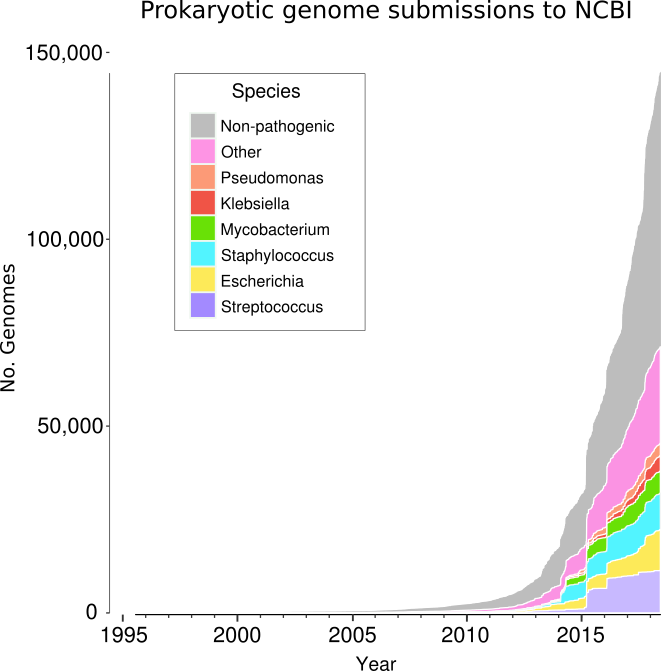
\includegraphics[scale=0.65]{intro/path_graph.png}
  \centering
  \caption[Total prokaryotic genome submissions to NCBI over time]{Total prokaryotic genome submissions to NCBI over time, showing the exponential growth in prokaryotic genome submissions. Data taken from the NCBI prokaryote genome assembly summary  (ftp://ftp.ncbi.nlm.nih.gov/genomes/GENOME_REPORTS/prokaryotes.txt, date range 1995-2018). Relative proportions of pathogenic species and strains identified as pathogenic by \cite{Ecker2005} are shown as coloured stacks grouped by genera, showing that the majority of prokaryotic genomes in NCBI are from pathogenic species. The top 6 genera are ordered by proportion from smallest to largest (\textit{Pseudomonas}, \textit{Klebsiella}, \textit{Mycobacterium}, \textit{Staphylococcus}, \textit{Escherichia} and \textit{Streptococcus}), with "Other" representing the combined sum of remaining pathogen genomes.}
  \label{fig:path_graph}
\end{figure}
Despite representing a tiny fraction of microbial diversity \citep{Balloux2017}, prokaryotic pathogens are over-represented within genome databases (Figure \ref{fig:path_graph}). Genera such as \textit{Streptococcus}, \textit{Escherichia}, and \textit{Salmonella} that contain multiple pathogenic species have been densely sampled, facilitating increasingly detailed and granular genomic studies of pathogenic bacteria.\par

Genomics, the study of genome sequences, is intertwined with the field of bioinformatics, which is tasked with both managing and interpreting these increasingly large amounts of sequence data. Early bioinformatics tools for biological sequence analysis were designed to assemble \citep{Dayhoff:1962:CCP:1461518.1461546,Staden1979} and compare \citep{NEEDLEMAN1970443,Smith_Waterman_1981,Thompson_Higgins_Gibson_1994,Felsenstein_1981} amino acid and nucleotide sequences, which may be simply represented as character strings in a computing context \citep{Gauthier2018-bk}.\par
Much of modern bioinformatics remains focused on these same problems; studying both the information content within, and comparisons between biological sequences. Detailed introductions to these methods can be found in numerous textbooks covering bioinformatics methods and algorithms, e.g \cite{Eddy_BSA_1998,Mount_2004} and \cite{Waterman_1995}.

\subsection{Next Generation Sequencing technologies}
The introduction of NGS technologies with massively increased capacity in the mid-2000’s has revolutionised the field of genomics. Current sequencing methods can be broadly split into ‘short’ and ‘long’ read technologies, depending on the size of fragments that can be sequenced. Most modern sequencing platforms use a ‘sequencing-by-synthesis’ approach, using nucleotides modified with dye molecules (dNTPs) which fluoresce at wavelengths specific to each nucleotide base \citep{Eid2009-gt,Bentley2008-xb}.\par
Short read sequencing technologies typically utilise dNTPs with reversible dye termination chemistry \citep{Bentley2008-xb,Croucher2009-iw}, which terminate strand extension upon incorporation. In Illumina short-read sequencing, individual fragments are first ligated and amplified on a substrate, generating clonal clusters of forward and reverse strands from the same sequence. During sequencing-by-synthesis, single dNTPs are incorporated, and the base is determined by excitation of the dNTP's fluorophore over a cluster of fragments, which is then cleaved prior the next cycle. This method of sequencing has a low error rate during base calling, but is limited to smaller fragments (50--500 nt). \par
Long-read technologies have no upper limit on molecule size and excel at resolving repetitive sequence regions, but require large amounts of DNA to produce enough data to compensate for high error rates. The SMRT\textsuperscript{TM} sequencing approach used by Pacific Biosciences uses a specialised DNA polymerase fixed to a substrate, and dNTPs with a fluorophore linked to the terminal phosphate that are cleaved during synthesis. This approach enables reactions to proceed rapidly, and produces a natural double-stranded DNA product \citep{Korlach2010-dj}. The dNTPs fluoresce as they approach the illuminated substrate and are incorporated into the new strand, enabling bases to be called \citep{Eid2009-gt}.\par
Another emerging class of long-read sequencing technologies detects nucleotides by measuring changes in electrical current as samples pass through protein nanopores embedded in a polymer membrane. Voltage is applied to the membrane, causing a current to pass through the nanopore \citep{Jain2016-hk,Feng2015-ut}. An affixed \textphi 29 DNA polymerase acts as a processive enzyme, ratcheting nucleotides through the pore one base at a time in a controllable reaction \citep{Cherf2012-jh}. Bases are determined by characteristic fluctuations in membrane potential with the passing of each nucleotide \citep{Stoddart2009-bo}. Each nanopore is part of a single circuit, allowing the current across individual nanopores to be controlled and measured.\par
Nanopore technologies such as the MinION sequencer have been an exciting development due to the small size and portability of the instrument, and its ability to produce extremely long (>140 kb) sequencing reads \citep{Jain2016-hk}. Improvements in both nanopore technology and assembly programs are generating high quality bacterial \citep{Quick2014-qr}, human \citep{Jain2018-xk} and even native RNA viral genomes \citep{Keller2018-sb}.\par

\subsection{Standard Bioinformatic analysis of NGS sequencing data}
Genomics is a rapidly changing field, both in terms of sequencing technologies and the bioinformatics tools used to analyse sequence data. While there are numerous tools and  workflows for processing sequencing data, bioinformatics pipelines generally include quality control of raw data, an alignment step for assembling reads or mapping reads to a reference sequence, and downstream quantitative or qualitative analysis.\par
Quality control of data using tools such as FastQC \citep{Andrews_2010} provide summary statistics that can identify problems with the data-set that originate from library composition or from the sequencing process. Typically some correction must be performed on the sequencing reads to remove any remaining sequencing adapters, or remove reads that are too short or that have missing sequencing pairs. For short-read sequencing data, trimming tools such as trimmomatic \citep{Bolger_Lohse_Usadel_2014} or cutAdapt \citep{Martin_2011} can remove regions of sequence below a certain quality score threshold. For long-read sequencing data, which contain randomly introduced errors, reads must be corrected by alignment of sequencing reads. This may be achieved by consensus overlay correction if there is sufficient read depth, or using additional short-read sequencing data, which have lower error rates.\par
Many sequencing projects involve an assembly step, which aims to reconstruct genomes or transcripts from sequencing reads. Assembly tools are a particularly active area within bioinformatics, as new software is rapidly developed, aiming to both reduce computational time and improve assembly quality \citep{Sohn_Nam_2018,Simpson_Pop_2015}. Common algorithmic approaches for assembly include de Bruijn graph-based methods for short read data, and alignment-based methods for long-read data \citep{Simpson_Pop_2015}.\par
For transcriptome analysis, reads must be assigned to their originating genome sequence by a process called mapping. The number of reads originating from a particular gene or genomic feature is then used to give a quantitative estimate of gene expression. Alignment tools such as BWA \citep{Li2009-cw} and Bowtie \citep{Langmead2012-xq} can align sequence reads to a reference genome. Downstream quantification tools can then be used to provide ‘counts’ of reads mapped for individual genes \citep{Li_Dewey_2011,Anders_Pyl_Huber_2015,Trapnell_Roberts_Goff_Pertea_Kim_Kelley_Pimentel_Salzberg_Rinn_Pachter_2012}. Alternatively, recent tools such as Kallisto \citep{Bray2016-oi} and Salmon \citep{Patro_Duggal_Love_Irizarry_Kingsford_2017} use k-mer based methods to rapidly align and quantify reads, using reference transcripts. A variety of statistical analysis  packages can then be used to interpret gene expression data, including DESeq2 \citep{Love2014-dv}, EdgeR \citep{Robinson_McCarthy_Smyth_2010} and Limma \citep{Ritchie_Phipson_Wu_Hu_Law_Shi_Smyth_2015}.\par
High-throughput pipelines for assembly and annotation are commonly used in bacterial genome sequencing projects \citep{Seemann_2014,Aziz_2008,Tatusova_DiCuccio_Badretdin_Chetvernin_Nawrocki_Zaslavsky_Lomsadze_Pruitt_Borodovsky_Ostell_2016}. These workflows implement a variety of tools to identify open reading frames \citep{Delcher_Bratke_Powers_Salzberg_2007,Hyatt_Chen_Locascio_Land_Larimer_Hauser_2010} and annotate genes based on homology to reference proteins or non-coding RNAs \citep{Punta_2012,Huerta_2017,Altschul1990-kr,Nawrocki_Infernal_2013,Nawrocki_Rfam_2015}.\par

\subsection{RNA-seq}
A revolutionary application of NGS technologies is the sequencing of RNA transcripts (RNA-seq). RNA-seq allows the transcription rate of a gene to be estimated by providing a snapshot of the population of transcribed RNAs present in a sample (transcriptome). Protocols for RNA-seq employ similar methods as short-read DNA sequencing, with an additional step where complementary DNA (cDNA) is synthesised from RNA transcripts prior to sequencing \citep{Wang2009-ao}.\par
As with DNA sequencing, RNA-seq technologies are rapidly developing, producing increasingly high-resolution transcriptomes \citep{Creecy2015-is}. Increases in sequencing capacity and depth allows low abundance transcripts to be detected, and stranded sequencing methods have been developed to determine the originating strand and orientation of a sequencing read \citep{Parkhomchuk2009-xj,Fullwood2009-wu}. Almost all current RNA-seq protocols are based on Illumina short-read sequencing, however, nanopore-based high-throughput RNA-seq technology is emerging \citep{Workman2018-bo}.\par 
In the past decade, a variety of novel technologies have emerged built on RNA-seq methods \citep{Saliba2017-ax,Hrdlickova2017-ty}. Improvements in library preparation can determine the transcriptomes of single cells (single-cell RNA-seq, or scRNASeq) \citep{Islam2014-rx}, enabling transcriptomic studies across whole tissues or populations of bacteria.\par 
Other technologies can shed light on the functional roles and fate of RNA molecules. Interactions between transcripts (RNA-RNA interactions) can be identified by cross-linking, ligating and sequencing RNA molecules participating in RNA duplexes \citep{Kudla2011-xi}. Alternatively, RNA duplexes can be purified by immunoprecipitation of enzymes which preferentially bind double-stranded RNA \citep{Lioliou2013-if}.\par
RNAs participating in complexes with RNA-binding proteins can be studied by gradient separation (GRAD-seq) \citep{Rederstorff2010-dr,Smirnov2016-yt} or UV-RNA-protein crosslinking \citep{Licatalosi2008-cm}, which can be combined with immunoprecipitation of specific RNPs of interest \citep{Zhao2010-nu,Lu2014-cg,Melamed2016-xv}. The dynamics of transcription initiation and termination can also be studied by selectively sequencing the 5$\textprime$  \citep{Sharma2010-lv} and 3$\textprime$  end of transcripts \citep{Dar2016-vm}, called TSS-seq and Term-seq respectively. \par
Increased depth of sequencing and improved mapping software has also enabled simultaneous studies of gene expression in bacterial pathogens and their host without the prior separation of samples \citep{Westermann2012-pr}. As the rapid pace of development of such technologies continues, we can expect RNA-seq to provide an increasingly nuanced and comprehensive view of gene expression.\par

\section{Bacterial ncRNAs in pathogens} 
Much of the focus of early molecular biology concerned proteins and their functions. It has since been found, however, that some RNA molecules directly enact specific biological functions both as functional components and regulators of transcription and translation \citep{Eddy2001-jv,Morris2014-mm} (Figure \ref{fig:central_dogma}). These RNA molecules, termed ‘non-coding RNAs’ or ncRNAs, are a heterogeneous class of genes which enact their function as RNA transcripts, and are found in all domains of life (Figure \ref{fig:central_dogma}). 
\begin{figure}[H]
    \centering
    \begin{minipage}[b]{0.47\linewidth}
  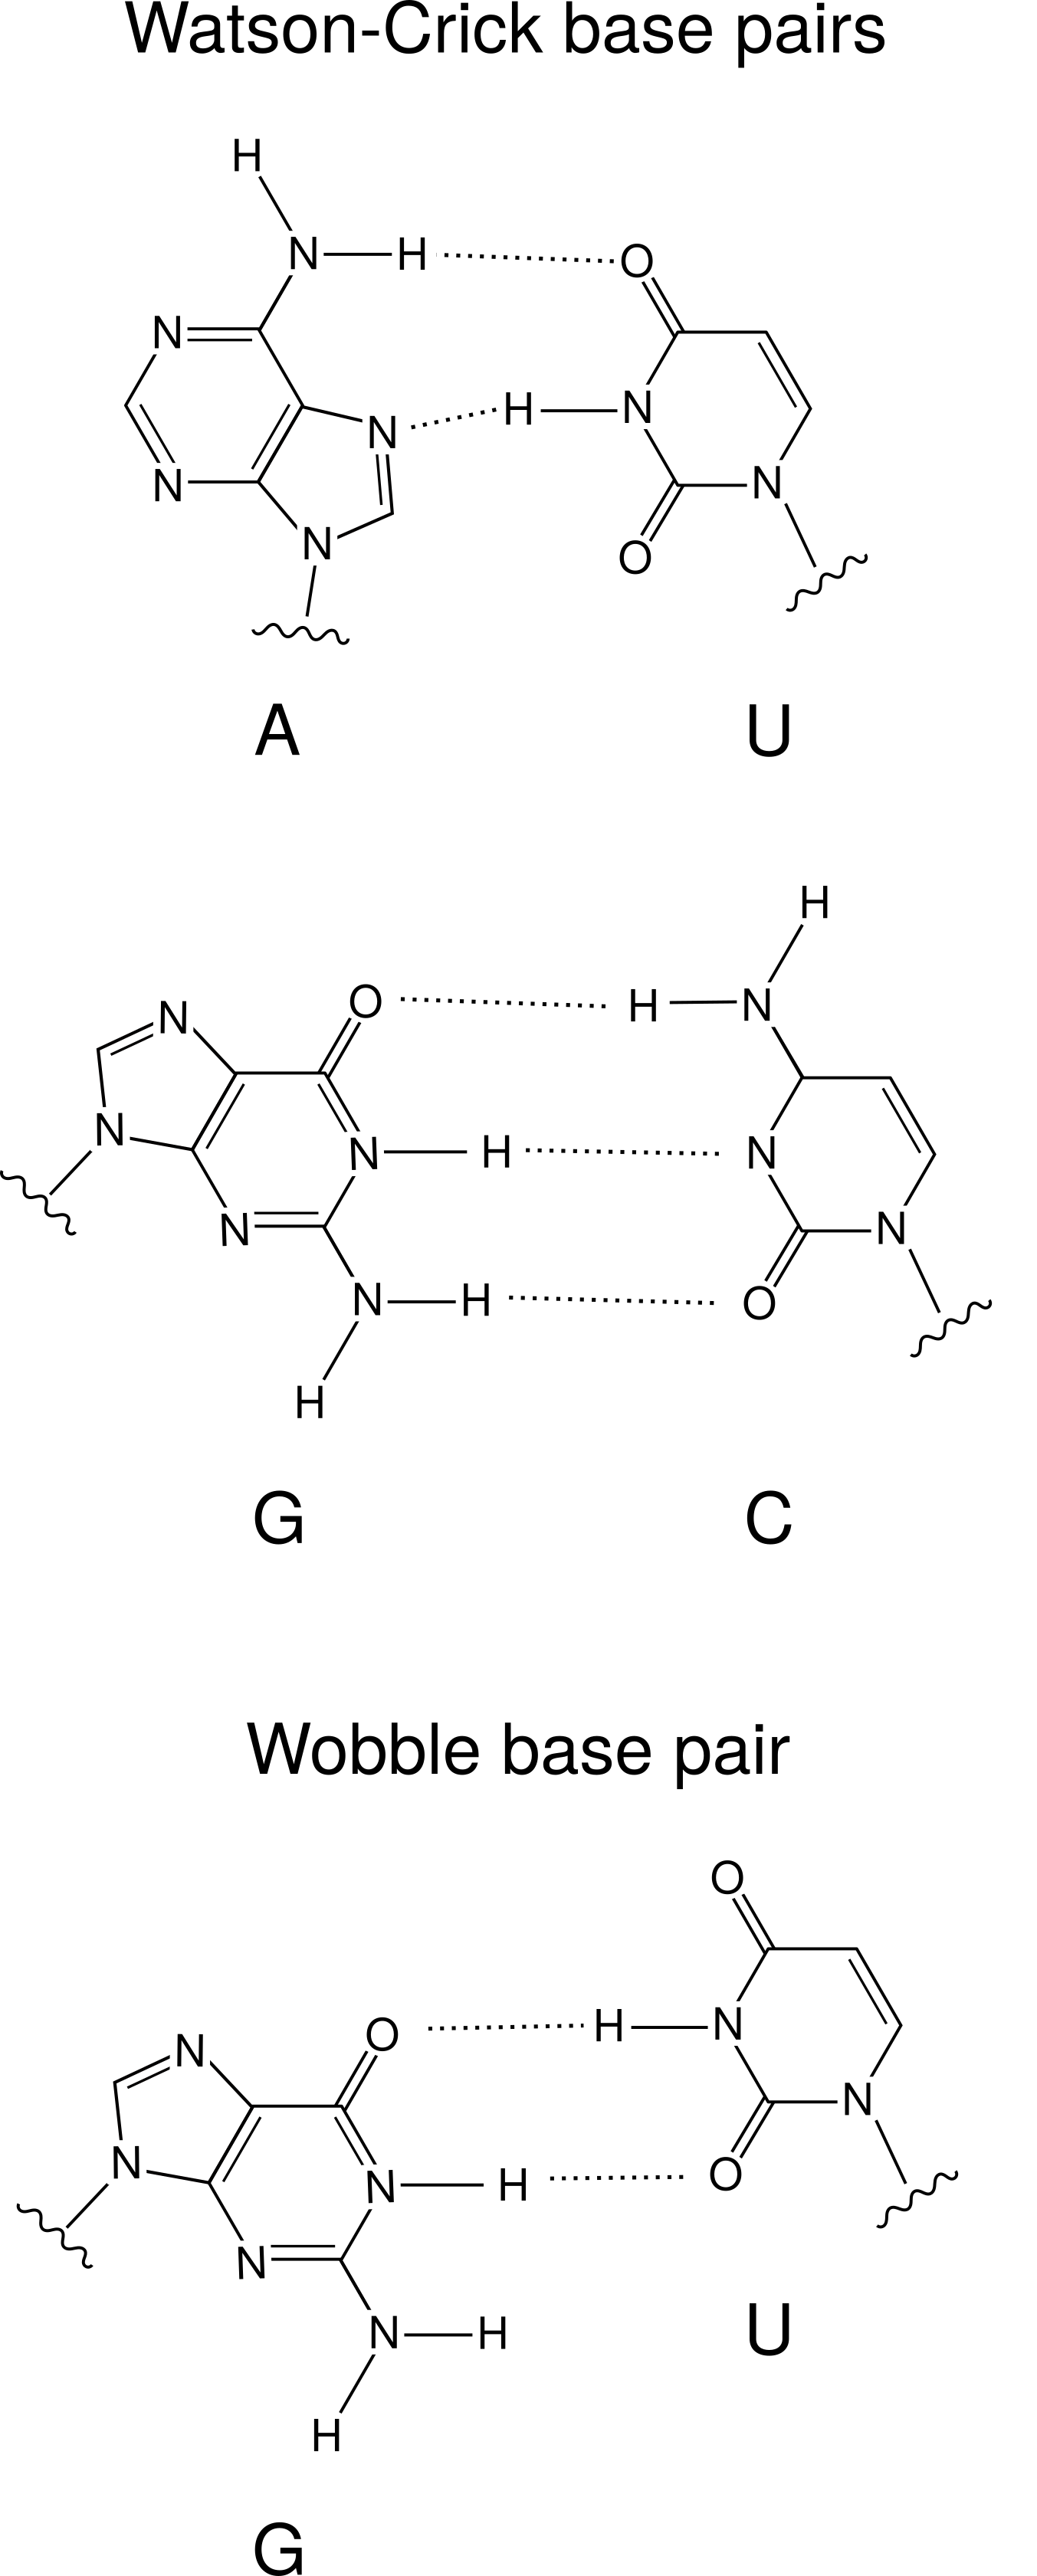
\includegraphics[scale=0.45]{intro/basepairing.png}
  \centering
  \caption[Nucleotide base pairs found in RNA secondary structures]{Nucleotide base pairs found in RNA secondary structures. \textbf{Top:} Watson-crick base pairs between Adenosine (A) and Uracil (U), and Guanine (G) and Cytosine (C). \textbf{Bottom:} Wobble base pair formed between Guanine and Uracil. Hydrogen bonds shown as dashed lines.}
  \label{fig:basepairs}
    \end{minipage}
\quad
    \begin{minipage}[b]{0.47\linewidth}
        \centering
          \includegraphics[scale=1.4]{intro/central_dogma.png}
  \caption[Roles of ncRNA regulation in different processes within the central dogma of molecular biology]{Roles of ncRNA regulation in different processes within the central dogma of molecular biology. Based on Figure 1, \cite{Wahlestedt2013-so}. }
  \label{fig:central_dogma}
        \par

          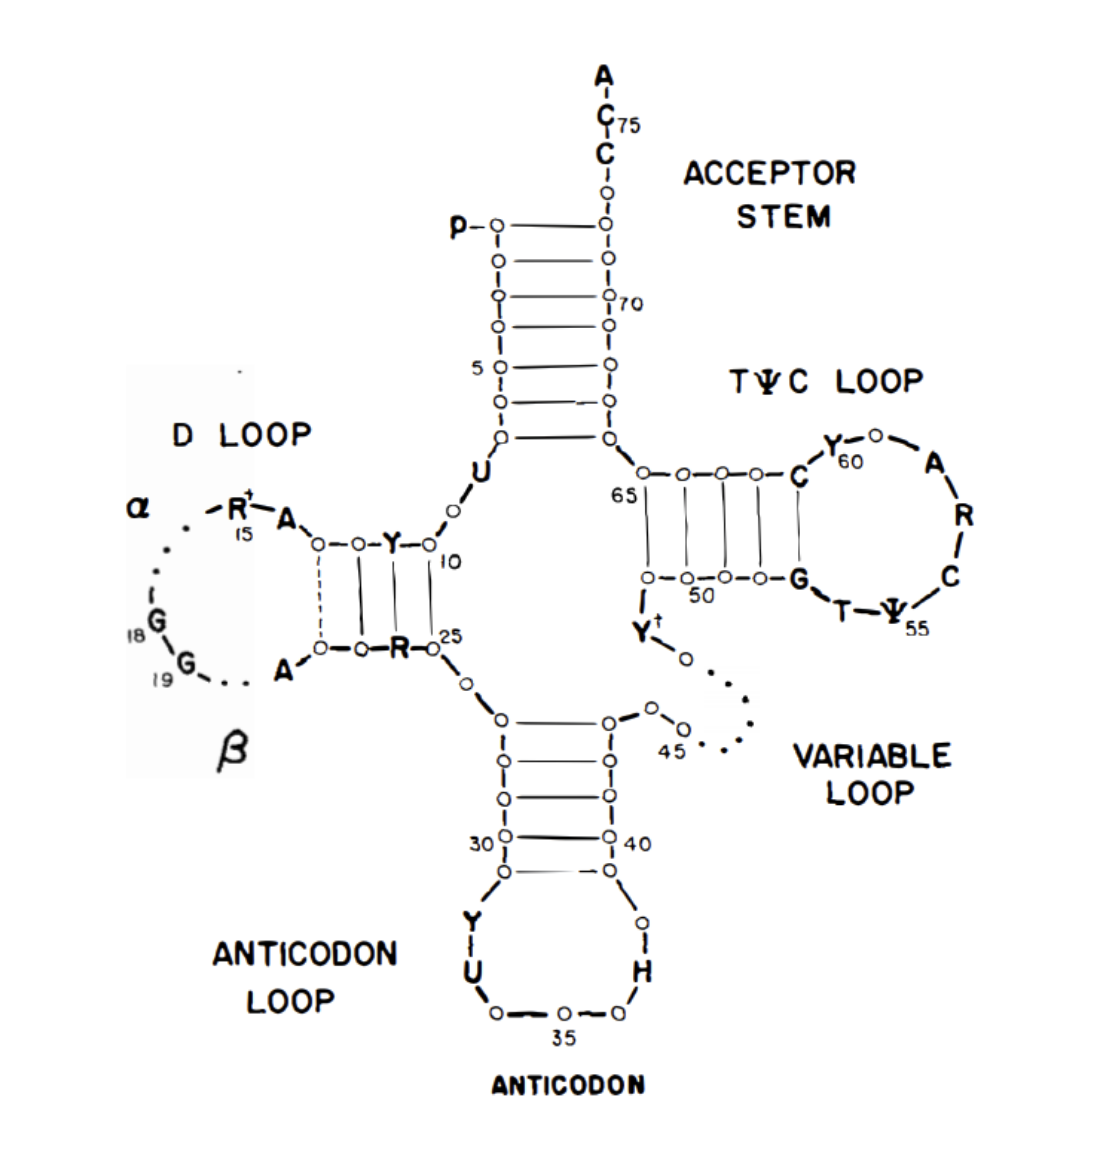
\includegraphics[scale=0.15]{intro/tRNA.png}
  \centering
  \caption[Example of an RNA secondary structure]{Example of an RNA secondary structure: Representation of base-pairing secondary structure of a tRNA. Taken from Figure 2, \cite{Rich1976-hs}.}
  \label{fig:tRNA}
    \end{minipage}
\end{figure}

Much like proteins, ncRNAs possess a diverse array of sizes, structure, function and modes of action. Many ncRNA transcripts form complex secondary and tertiary structures \textit{via} intramolecular base pairing (see Figure \ref{fig:basepairs} and Figure \ref{fig:tRNA}), which is the functional determinant of many ncRNAs. \par

Non-coding RNAs can be broadly grouped into three functional categories: catalytic RNA (ribozymes), RNAs which participate in ribonucleoprotein complexes (RNPs), and regulatory ncRNA \citep{Cech2014-pe}. Famous examples of ncRNAs include ubiquitously conserved elements of the translation machinery, such as the ribosome, tRNAs (Figure \ref{fig:tRNA}), and the RNase P ribonuclease involved in tRNA processing. Other ribozymes found in bacteria include Group I and II introns \citep{Lambowitz2011-oq,Hausner2014-ud}, which are self-splicing ribozymes that self-propagate in many lineages.

Aside from ribosomes, few RNPs are known in bacteria. Notable examples include the highly conserved 6S RNA, which binds with \textsigma70-RNA polymerase with widespread effects on transcriptional regulation \citep{Wassarman2007-de}, the transfer-messenger RNA (tmRNA) that recycles stalled ribosomes and their associated mRNAs and protein products \citep{Moore_Sauer_2007}, the signal recognition particle (SRP) RNA involved in protein transport and localisation \citep{Akopian_Shen_Zhang_Shan_2013}, and the CRISPR-Cas protein-RNA complex which recognises and guides endonucleases to foreign DNA \citep{Barrangou2015-sf}.\par

\subsection{Gene regulation in pathogens}

As single-celled organisms, bacteria must dynamically control internal concentrations of macromolecules in order to respond to changes in the local environment \citep{Dorman2018-dv}. While a handful of genes involved in processes essential to life are constitutively expressed, bacterial genomes also contain cohorts of genes that contribute most to fitness when expressed under specific growth conditions \citep{Price2016-gi}. Effective gene regulation increases fitness by preventing detrimental epistasis, and by allocating resources appropriately. \par

Bacterial pathogens face additional stresses during infection as they must traverse through radically different environments both outside and inside the host, each with its own set of stressors \citep{Cotter2000-it}. Virulence genes, such as those involved in toxin secretion or adhesion to host cells, must also be tightly controlled for maximum effect. Gene regulation therefore directly influences pathogenicity. \par 
In addition to gene regulation by transcription factors and changes in DNA and RNA conformation or topology, advances in RNA biology have revealed complex and sophisticated regulatory roles of ncRNA in gene regulation in bacteria \citep{Hor2018-ns}.

\subsection{Regulatory ncRNA}

Regulatory RNAs are a diverse class of ncRNA whose roles as regulators at transcription, translation and at the protein level are being increasingly appreciated \citep{Cech2014-pe}. Regulatory RNAs were initially discovered in the 1980’s, mostly as antisense regulators of plasmid replication proteins in \textit{Escherichia coli} \citep{Conrad1979-xe,Stougaard1981-np,Inouye1988-rv}. Although the 6S RNA was technically the first regulatory ncRNA discovered \citep{Brownlee1971-lh}, its exact function remained unknown until decades later \citep{Barrick2005-if}. Few regulatory ncRNAs were discovered until the early 2000’s, but since then a wide variety of bacterial ncRNAs have been found that contribute to pathogenicity through versatile mechanisms \citep{Papenfort2010-cj}.\par

Interesting examples of bacterial ncRNAs include \textit{cis}-regulatory elements such as riboswitches, which are structured elements that change conformation to allow or deny the translation of the downstream coding sequence. Most known examples of riboswitches act as sensors, detecting metabolite ligands to self-regulate biosynthetic pathways \citep{Serganov2013-fz}. A particularly elegant example of a riboswitch involved in pathogenicity is the \textit{prfA} thermoswitch of \textit{Listeria monocytogenes}, which unfolds at 37°C to allow the translation of Prfa, a transcriptional activator of virulence genes \citep{Johansson2002-ar}.\par

\subsubsection{Bacterial small RNAs} 

Bacterial sRNAs are a broad and heterogeneous class of ncRNAs that regulate gene expression by interacting with both mRNA and proteins (Figure \ref{fig:sRNA_cis_trans}). These small (\textasciitilde50--500 nt) transcripts are often expressed only in specific growth conditions, which gives bacteria an effective toolkit to fine-tune protein expression to their needs.\par
The majority of characterised sRNAs act by an antisense binding mechanism. These transcripts can base-pair with their targets to various extents in order to degrade, stabilise or enhance transcription of mRNAs, or sequester or inhibit proteins by targeting RNA-binding sites \citep{Storz2011-tb,Barquist2015-pa} (Figure \ref{fig:lars_fig.png}). Antisense sRNAs may be broadly classified into two categories: firstly, ‘\textit{cis}-acting’ or ‘\textit{cis}-antisense’ sRNAs, that are expressed from the opposite strand overlapping with their target protein, giving extensive complementarity for mRNA-sRNA interactions. Few \textit{cis}-antisense sRNAs have been extensively characterised, in part due to technical difficulties in discerning antisense transcription \citep{Georg2011-ee}. Many have been discovered as part of Type I toxin-antitoxin addiction modules, where they are transcribed opposite to toxin protein and prevent host death by sRNA-toxin mRNA inhibition \citep{Brantl2012-ad}. \par

A second type of antisense sRNAs, the ‘\textit{trans}-acting’ or ‘intergenic antisense’ sRNAs, are transcribed from intergenic sequences and tend to have smaller regions of complementarity (6--25 nt) with their targets. Many \textit{trans}-acting sRNAs interact with RNA chaperones to facilitate or stabilise sRNA-mRNA base-pairing interactions which would otherwise be weak or transient. The most well studied sRNA chaperone is the Hfq protein found in many gram-negative bacteria, but similar regulatory roles have recently been discovered in ProQ and FinO \citep{Attaiech2017-ip}. A handful of sRNAs have also been found to interact directly with proteins, either by competitive inhibition \citep{Babitzke2007-bb} or by encouraging dimerisation \citep{Duss2014-rs}.\par
\vspace{4mm}
\begin{figure}[H]
  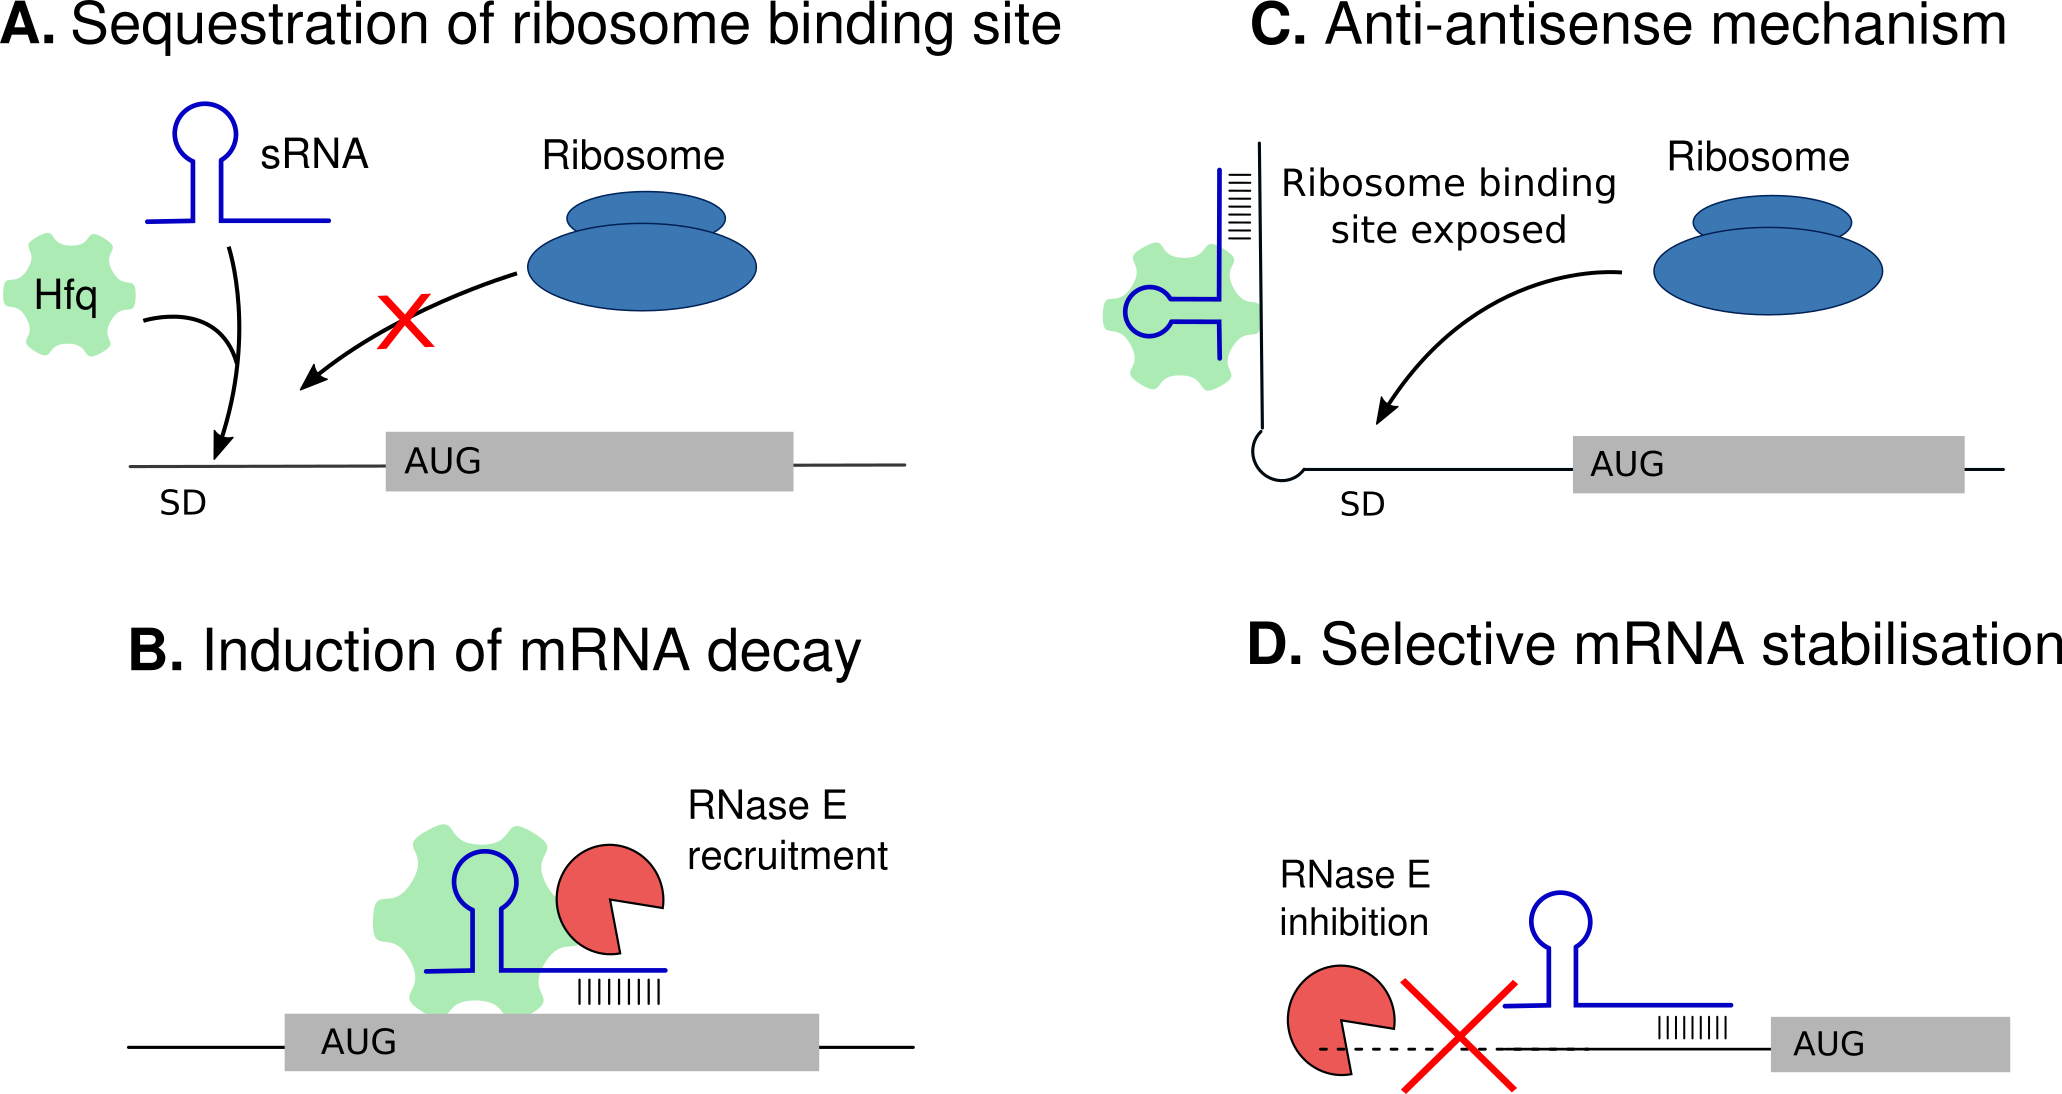
\includegraphics[scale=0.8]{intro/lars_fig.png}
  \centering
  \caption[Mechanisms of antisense sRNA regulation of mRNA]{Mechanisms of antisense sRNA regulation of mRNA. Antisense sRNAs may decrease protein expression by \textbf{(A)} binding to the Shine-dalgarno (SD) region of the target mRNA, preventing the mRNA from being loaded into the ribosome, or \textbf{(B)} inducing mRNA decay by recruiting RNase E. Conversely, sRNA binding may increase protein expression by \textbf{(C)} causing a conformational change in the mRNA that exposes a ribosome binding site or \textbf{(D)} increasing mRNA stability by preventing degradation. These interactions may be stabilised by the RNA chaperone protein Hfq. Adapted from \cite{Barquist2015-pa}.}
  \label{fig:lars_fig.png}
\end{figure}

Bacterial sRNAs may contribute to virulence by regulating the timing of virulence gene expression; either by direct activation/repression, as part of a larger regulatory circuit, or through multiple routes, such as the \textit{Salmonella} sRNA IsrM which attenuates an effector and \begin{wrapfigure}{r}{0.45\textwidth}
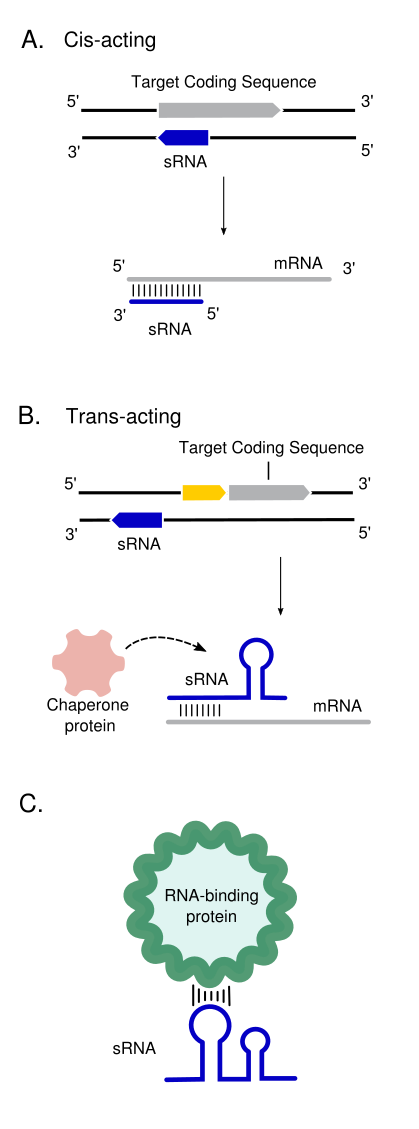
\includegraphics[scale=1.5]{intro/sRNA_cis_trans.png}
  \centering
  \caption[Examples of antisense sRNA types and functions]{Examples of antisense sRNA types and functions. \textbf{A.} A \textit{cis}-acting sRNA is expressed antisense to a protein coding sequence. The transcribed sRNA then base-pairs extensively with the mRNA of the target gene. \textbf{B.} A \textit{trans}-acting sRNA gene is transcribed from a region distal to its target. The transcribed sRNA then interacts with the target mRNA, utilising a chaperone protein to stabilise the small antisense binding region. \textbf{C.} A \textit{trans}-acting sRNA interacts with the RNA-binding site of an RNA-binding protein to inhibit or sequester the protein. Figure loosely based on Figure 1 from \cite{Pernitzsch2012-xo}.}
  \label{fig:sRNA_cis_trans}
\end{wrapfigure} its corresponding virulence regulator \citep{Gong2011-vs}.\par
Small RNAs involved in virulence have been found in diverse roles such as adhesion, motility \citep{Vannini2016-mn}, toxin secretion and biofilm formation \citep{Bradley2011-rh}. Many sRNAs involved in virulence are found in horizontally acquired mobile elements and pathogenicity islands \citep{Papenfort2010-cj}.  
These sRNAs may control genes within the same element, or interact with the core genome. An example of the latter is \textit{Salmonella} pathogenicity island sRNA InvR, which controls membrane protein expression during cell invasion \citep{Pfeiffer2007-yb}. \par

Many sRNAs are also involved in the regulation of stress responses and cell survival either through a global stress response or interactions with individual genes \citep{Bhatt2016-dk,Hoe2013-kh}. Some sRNAs involved in stress responses also contribute to virulence. An example of this can be seen with the \textit{Salmonella} RaoN and \textit{Pseudomonas aeruginosa} PesA sRNAs. Both of these transcripts function generally within the oxidative stress response, that also benefit the bacterium’s survival within the host. RaoN is required for replication within macrophages  \citep{Lee2013-un}; PesA is induced in low oxygen conditions and temperatures that may be encountered in the host \citep{Ferrara2017-su}.\par

The small binding sites of many sRNAs adds flexibility to regulatory networks, as relatively few changes are required to alter the sRNA target range (regulon). An example of regulon reshaping in virulence can be seen in the conserved paralogues \textit{glmY} and \textit{glmZ}. In \textit{E. coli} these sRNAs are part of the core genome in both pathogenic and non-pathogenic strains, however, the GlmY/Z regulon includes virulence genes when these sRNAs are present \citep{Bhatt2016-dk,Gruber2015-rb}. \par

Finally, an example has been found of an sRNA which affects host cells. The \textit{Salmonella} Typhimurium sRNA PinT is expressed within the host cell and both controls the expression of \textit{Salmonella} virulence factors and affects JAK-STAT signalling in the host transcriptome \citep{Westermann2016-mr}.


\section{ncRNA discovery and annotation}
The rate of discovery of ncRNAs has lagged behind that of proteins for several reasons. Most ncRNAs are small molecules, typically shorter than the mRNAs of protein-coding genes. Early ncRNA discovery was a laborious process, where ncRNAs were isolated by size-separation of RNA fractions using sucrose gradients, gels and radioactive labelling \citep{Andersen1987-tn}. Many ncRNAs are also difficult targets for classical mutagenesis due to their size and tolerance of mutations \citep{Gottesman2004-ke}, the presence of paralogues, and functional redundancy within complex regulatory networks. Bioinformatics approaches are also used to identify and study ncRNA genes. However, unlike proteins, several properties of ncRNAs make them difficult to identify from genome sequence alone. Firstly, ncRNA genes lack shared, recognisable sequence motifs, such as stop/start codons or long open-reading frames found in protein-coding genes. Secondly, many ncRNAs exhibit poor conservation, and instead tend to preserve base-pairs that contribute to structure \citep{Rivas2001-lk}.

\subsection{Experimental techniques}
Historically, regulatory ncRNAs were discovered by chance \citep{Thomason2010-ax}. Large numbers of ncRNAs were not discovered until the development of tiling microarrays that could screen for expressed intergenic regions \citep{Gottesman2004-ke}. Phenotype assays of sRNA deletion mutants have also been used to identify the importance of sRNAs to organismal fitness in different growth conditions \citep{Hobbs2010-lj,Santiviago2009-hn}. Most of these techniques have now been largely superseded by RNA-seq. Multi-condition transcriptomics are becoming standard for identifying sRNAs. The most notable of these to date have used over a dozen separate growth conditions to comprehensively screen for sRNAs in \textit{E. coli} \citep{Rau2015-gt} and \textit{Salmonella} Typhimurium \citep{Kroger2013-pg}.\par
Several RNA-seq based methods for studying gene fitness and RNA interactions have been applied to bacterial sRNAs. Some sRNA-specific methods have also recently been developed which utilise Hfq-based assays to detect Hfq-sRNA interactions \citep{Holmqvist2016-xhj}, or to enrich sRNAs ligated to target mRNA \citep{Melamed2016-xv}. Others can identify novel sRNA chaperones by crosslinking known sRNAs attached to proteins \citep{Smirnov2016-yt}. Transposon insertion sequencing (Tn-Seq or TraDIS), which probes the genome for genes that are essential for growth, is also a useful way to determine functional intergenic regions and validate the contribution of sRNAs to fitness in a specific growth condition \citep{Van_Opijnen2009-ns,Barquist2013-ili}. \par  
RNA structure determination is another important step in understanding transcript stability and function. Several methods use structure-dependent covalent modifications of nucleotides. An example of this is SHAPE-seq, which modifies bases that are structurally flexible (and hence less likely to participate in secondary structure) which are then detected by RT-PCR as the modified base inhibits primer extension \citep{Tyrrell2013-ww,Watters2016-dm}. PARIS, another technique, can globally determine RNA-RNA interactions and local regions of secondary structure by cross-linking double-stranded RNA, which is then purified and sequenced \citep{Lu2016-qk}. INTERFACE provides an alternative approach, by surveying regions of ncRNAs that are not participating in secondary structure. This technique uses a reporter system that attenuates transcript elongation when RNA probes are not hybridised \citep{Mihailovic2018-kv}.

\subsection{Prediction from genomic sequence}
Although ncRNAs have few distinguishable features at the sequence level, several approaches have been attempted to predict ncRNAs \textit{de-novo} by comparative genomics. Several ncRNAs were discovered by early comparative genomics studies, which looked for conserved intergenic regions with signals of transcription, such as promoters and terminators \citep{Argaman2001-oc,Wassarman2001-ht}. Subsequent tools analysed nucleotide substitution patterns within alignments to predict protein-coding potential and look for signals of RNA secondary structure conservation, or the maintenance of thermodynamic stability \citep{Gruber_2010,Pedersen_2006,Rivas2001-lk}.

Conversely, comparative genomics has focused on identifying ncRNA-like sequences in intergenic regions within poorly conserved genomic islands, which are often sources of species or genus-specific genes involved in pathogenicity \citep{Padalon-Brauch2008-bp}. Promoter and terminator predictions within individual genomes can be used to predict candidate intergenic ncRNAs, where confident promoter models are available \citep{Sridhar_2010,Herbig_Nieselt_2011}. A study by \cite{Klein2002-fm} used sequence composition to identify structured ncRNAs, which often have GC-rich sequence compositions, against a background genomic AT bias in thermophilic bacteria.

\subsection{ncRNA homology search}

Non-coding RNAs are generally much more poorly conserved than proteins at the sequence level \citep{Lindgreen2014-dk}. As homology search relies on sequence alignment, homology search techniques for ncRNA are generally less effective than for proteins \citep{Sun2012-ef,Rivas2001-lk,McGimpsey2019-ys}.

BLAST is the most widely used tool for nucleotide homology search, and one of the most highly cited scientific papers \citep{Altschul1990-kr}. BLAST is based on a modified Smith-Waterman heuristic pairwise alignment algorithm --- homology is determined by finding the optimal alignment of pairs of sequences, factoring in penalties for substitutions, gaps and indels.

More recently developed homology search tools incorporate multiple sequence alignments, and are more effective at determining homologous but divergent sequences \citep{Park1998-lu,Lindahl2000-ra}. One such approach is profile hidden Markov model (profile HMM) homology search. Profile HMMs are built from a trusted multiple sequence alignment, and are statistical models that incorporate at each point in a sequence the probability that there is a specific residue, a deletion, or an insertion. By aligning sequences against profile HMMs, more divergent sequences can be detected. Profile HMMs have been shown to be effective for investigating deeply conserved protein \citep{Madera2002-mk} and nucleotide sequences across large phylogenetic distances \citep{Freyhult2007-gz}, and tools like the HMMER \citep{Eddy2009-hmmer} suite of programs can utilise profile HMMs for effective protein and nucleotide homology search \citep{Eddy2011-hi}.\par

RNA structure is important for the function of many ncRNAs, and base-pairs which contribute to functional components of secondary structure may be more conserved than the underlying nucleotide sequence. Multiple sequence alignment tools have low efficacy for structured RNAs with low sequence similarity (50--60\%) \citep{Gardner2005-la}, which is a limiting factor for homology search. 

The incorporation of structural predictions by RNA-folding software can be used to improve homology search. Early tools to predict RNA secondary structure aimed to maximise the number of base pairs from single primary sequences, and hence identify the most thermodynamically stable secondary structure \citep{tinoco1971,tinoco1973,Nussinov1980-ka}. This approach was subsequently modified to use a nearest-neighbour energy model that captures additional information from stacked base-pairs \citep{Zuker1981-er}. Modern RNA folding tools use multiple sequence alignments to incorporate nucleotide or base-pair conservation as a predictor of structure \citep{Bujnicki_2013}. This may be done by two approaches: folding a multiple sequence alignment, or folding individual sequences and aligning secondary structures \citep{Gardner2004-uo}. 

Covarying base pairs, where complementary mutations occur to maintain structurally important base pairs, can be incorporated into covariance models as a measure of conserved secondary structure. Covariance models can compensate for large differences in sequences that may occur over large divergence times or due to loose constraints on sequence. While covariance models are the most effective method for ncRNA homology search \citep{Freyhult2007-gz}, they require the query ncRNA to have a conserved secondary structure, excluding ncRNAs with weak associations between structure and function \citep{Peterman2014-cs,Rivas2017-lg}.\par 

\section{Thesis Outline}

Recent studies have shown that sRNA sequence evolution is likely to be rapid, with many genes appearing to be species or even strain specific. However, it is difficult to ascertain whether this is due to rapid generation and loss of sRNA genes or due to the limitations of nucleotide homology search. Chapter Two presents a published review discussing the potential evolutionary origins of bacterial sRNAs, and the mechanisms by which new sRNA genes may arise \textit{via} the capture of transcriptional noise. Chapter 3 describes an approach to measure the conservation of \textit{Salmonella} sRNAs across the Enterobacteriaceae, and compares the phylogenetic distribution of sRNAs with their predicted evolutionary origins, which are estimated by conservation patterns and flanking proteins. This work demonstrates that many poorly conserved sRNAs are ‘new’ to the \textit{Salmonella} lineage, and have been introduced by mobile genetic elements. \par

Many sRNAs are only expressed under specific growth conditions, enabling careful timing of environmental responses in bacteria. \textit{Pseudomonas syringae} pv. \textit{actinidiae} (\textit{Psa}) is a plant pathogen which causes kiwifruit canker disease, and has had a significant impact on kiwifruit agriculture worldwide. Transcriptomes of \textit{Psa} grown \textit{in vitro} in multiple growth mediums were generated for this thesis by collaborators at Plant and Food Research, Auckland, NZ. In Chapter 4, these transcriptomes are used to study changes in gene expression relevant to pathogenicity between \textit{in vitro} samples, and also compared to another data-set of \textit{Psa} grown \textit{in planta}. In Chapter 5, this \textit{in vitro} and \textit{in planta} transcriptomes are also used to annotate potential ncRNAs in \textit{Psa}. Methods developed for sRNA homology search in Chapter 3 are used to measure candidate ncRNA conservation across \textit{Pseudomonas} genomes. Conservation, structural predictions and expression patterns are used to rank candidate ncRNAs, aiming to find genes that function in virulence. Finally, other work on two bacterial genome assembly and comparison projects is briefly described. 
\bibliographystyle{otago}
\bibliography{intro}

%\centering
%    \includegraphics[scale=1.4]{in%tro/central_dogma.png}
%  \caption[Roles of ncRNA %regulation in different processes within the central dogma of molecular biology]{Roles of ncRNA regulation in different processes within the central dogma of molecular biology (Based on Figure 1, \cite{Wahlestedt2013-so}). }
 % \label{fig:central_dogma}
%\end{wrapfigure}In the original central dogma of molecular biology, 
%  \centering

%RNA structure is important for the function of many ncRNAs, and base-pairs which contribute to functional components of secondary structure may be more conserved than the underlying nucleotide sequence.